\label{1_introducao}

A resolução de diversos problemas se dá na forma de algoritmos, de instruções bem definidas. No entanto, alguns algoritmos podem pedir inúmeras instruções até concluírem, o que pode até mesmo inviabilizar a solução encontrada. A Inteligência Artificial pode atuar sobre tais problemas de modo a interagir com o problema e aprender com ele a encontrar uma solução. Ótimos candidatos para esta tarefa são os chamados \emph{Algoritmos Evolutivos (AE)}.

Algoritmos evolutivos são aqueles que se baseiam nos princípios de evolução natural da Biologia, e são aplicados em um modo particular de solução de problemas: o da tentativa-e-erro. Tais algoritmos seguem um framework mais ou menos comum, atuante sobre diferente \emph{gerações} de um problema, por meio de mudanças e combinações de \emph{indivíduos} existentes numa \emph{população} \cite{eiben2003introduction}. Tal framework, conjuntamente com as ações evolutivas, pode ser visto na figura \ref{fig:evolution-framework}.

\begin{figure}[ht!]
    \centering 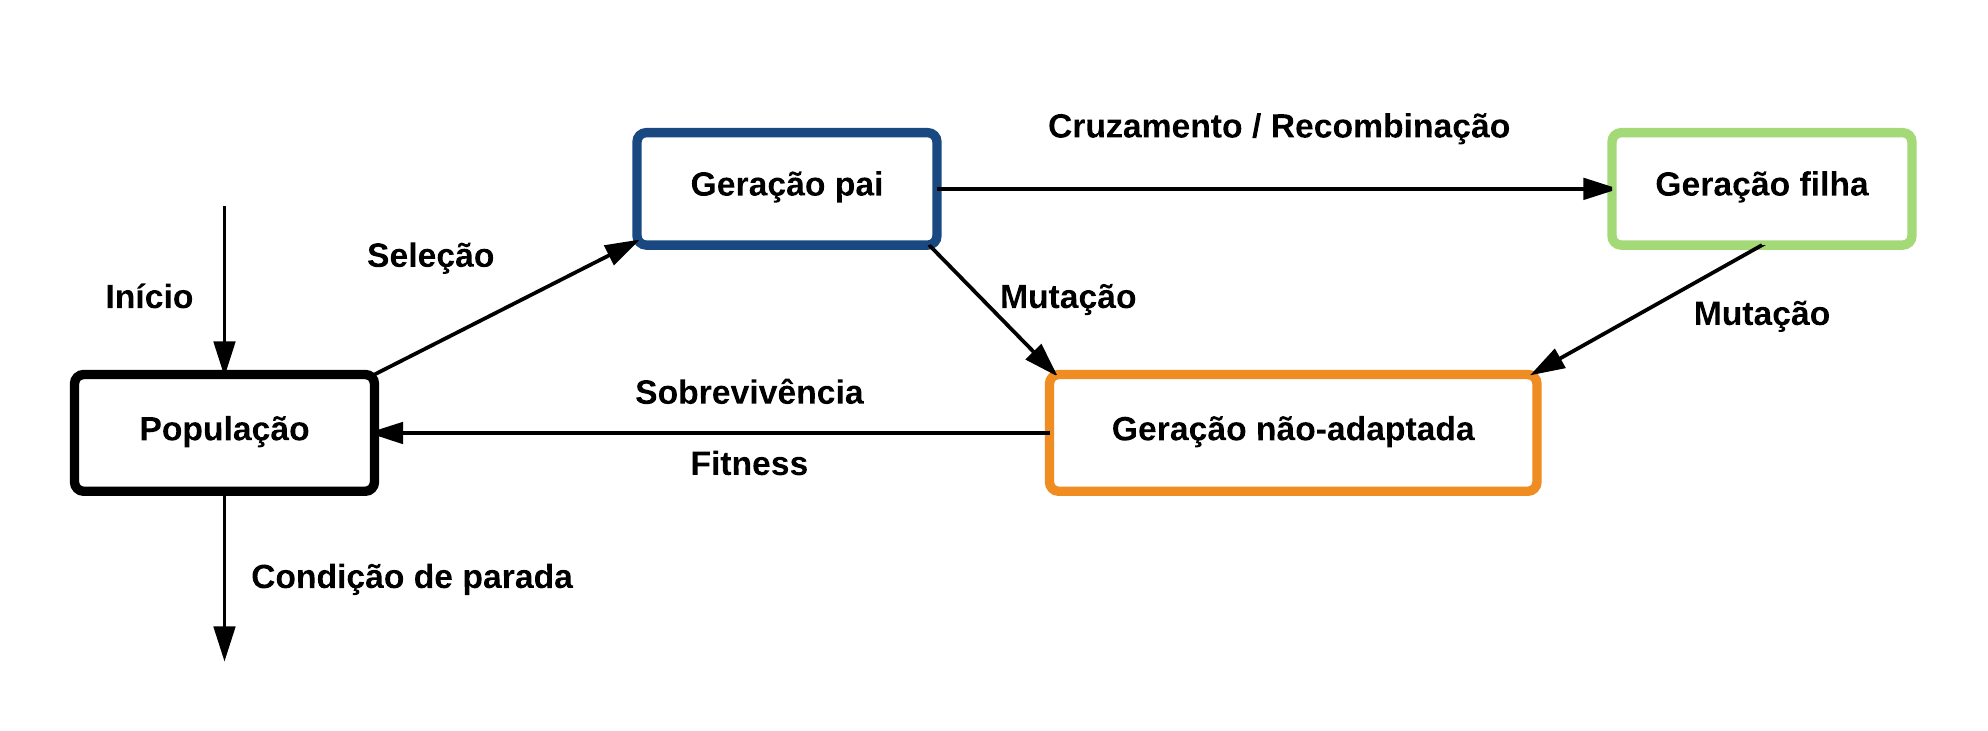
\includegraphics[width=1.0\textwidth]{evolution-framework.png}
    \caption{Framework de um algoritmo evolutivo.}
    \label{fig:evolution-framework}
\end{figure}

Cada indivíduo está tentando resolver o problema durante a execução do algoritmo evolutivo. A população contém estes indivíduos e é o alvo de interesse do processo evolutivo, e uma geração é a população que sobrevive após um ciclo de processos evolutivos do \ac{AE} sobre o problema. Similar ao processo evolutivo, seus componentes principais são as operações de variação (mutação e recombinação) e de seleção (seleção da geração pai e sobrevivência), chamadas aqui simplesmente de \emph{operações de evolução} \cite{eiben2011parameter}.

Este trabalho se utilizou de um grupo específico de Algoritmo Evolutivo, chamado de \textbf{Algoritmo Genético (AG)}. Um AG possui, como a menor estrutura de seus indivíduos, o \emph{gene}. Um gene costuma ter apenas duas propriedades: uma expressividade, normalmente associada a um valor numérico, e uma forma de mudá-la aleatoriamente.

Para um AG, a \emph{mutação} é uma mudança não controlada de um indivíduo feita a partir da mudança na expressividade de um ou mais genes. A \emph{recombinação} envolve a mistura de genes vindos de dois indivíduos que são cruzados. A \emph{seleção} envolve uma escolha a dedo dos melhores exemplares para cruzamento (a geração pai). A \emph{sobrevivência} envolve a rejeição de indivíduos que não estejam aptos o suficiente para resolver o problema. Tal aptidão é normalmente associada a uma função definida conjuntamente com o problema, chamada de \emph{função de fitness}.

\section{Objetivo}

Este trabalho propôs implementar um algoritmo genético capaz de resolver problemas determinados de diferentes complexidades e encontrar boas soluções após uma quantidade razoável de gerações.

\section{Abordagem}

Em termos de implementação, o AG deve ser tal que, uma vez aplicado sobre um problema e uma população, as gerações se desenvolvam automaticamente. O trabalho foi então dividido em 4 etapas:

\begin{enumerate}[label={[\arabic*]}]
	\item Escolha e implementação de problemas compatíveis com a aplicação do AE;
	\item Implementação do AG e de suas operações de evolução;
	\item Otimização do AG;
	\item Análise de performance e coleta de dados.
\end{enumerate}

As primeiras duas etapas são interdependentes, e precisaram ser completadas primeiro e conjuntamente. As demais etapas foram feitas sequencialmente, e foi encima da última etapa que as conclusões foram feitas.

De modo a permitir a reutilização deste código em outros problemas, o AG foi feito de modo a ser compatível com mais de um problema. As ferramentas de análise e coleta de dados consideraram tanto métricas comuns da literatura quanto parâmetros específicos dos problemas abordados.

Optou-se por utilizar Python como linguagem principal do código feito para este trabalho.

\section{Plano de Trabalho}
\label{sec:plano_trabalho}

Este trabalho foi planejado de forma que as etapas de otimização e análise do AE demorassem mais tempo. A validação dos resultados foi feita com base na literatura encontrada e nos resultados obtidos por algoritmos de código aberto (\emph{open source}) aplicados aos mesmos problemas.

\section{Organização do Trabalho}

\begin{itemize}
	\item \textbf{Capítulo 1:} Introdução
	\item \textbf{Capítulo 2:} Problemas Escolhidos
	\item \textbf{Capítulo 3:} Algoritmo Genético
	\item \textbf{Capítulo 4:} Otimização do Algoritmo
	\item \textbf{Capítulo 5:} Análises e Resultados
	\item \textbf{Capítulo 6:} Conclusões e Trabalhos Futuros
\end{itemize}
